\section{Introducción}

La práctica 6 estudia fenómenos observacionales que diferencian los modelos
geocéntrico y heliocéntrico: las fases y el tamaño angular de Venus, y el
movimiento retrógrado de Marte.
Aunque la guía original plantea el seguimiento con \textit{Stellarium}, en este
trabajo se usó un enfoque reproducible basado en consultas directas al sistema
\textit{NASA/JPL Horizons} mediante \texttt{astroquery} \citep{Ginsburg2019,Park2021}.

\section{Objetivos}

\subsection{Objetivo general}

Analizar cuantitativamente los tamaños y movimientos aparentes de Venus y Marte
para evaluar su consistencia con el modelo heliocéntrico.

\subsection{Objetivos específicos}

\begin{itemize}
  \item Calcular el período sinódico de Venus y Marte a partir de sus períodos sidéreos.
  \item Relacionar la fracción iluminada de Venus con su diámetro angular aparente.
  \item Identificar y medir el intervalo de retrogradación de Marte alrededor de la oposición 2027.
  \item Interpretar los resultados en términos de geometría orbital heliocéntrica.
\end{itemize}

\section{Marco teórico}

\subsection{Período sinódico}

El período sinódico $P_{\text{syn}}$ es el intervalo entre dos configuraciones
geométricas consecutivas observadas desde la Tierra. Se calcula como
\citep{Portilla2001,Karttunen2007}:

\begin{equation}
\frac{1}{P_{\text{syn}}}=\left|\frac{1}{P_{\text{planeta}}}-\frac{1}{P_{\oplus}}\right|.
\label{eq:psyn}
\end{equation}

\subsection{Venus: fases y tamaño angular}

Para Venus (planeta interior), la fracción iluminada depende del ángulo de fase
$\alpha$:
\begin{equation}
k=\frac{1+\cos\alpha}{2}.
\label{eq:k}
\end{equation}

El tamaño angular aparente escala aproximadamente como $\theta\propto 1/\Delta$,
donde $\Delta$ es la distancia geocéntrica. Por ello, cerca de conjunción
inferior Venus aparece grande y poco iluminado, y en conjunción superior aparece
pequeño y casi completamente iluminado \citep{Karttunen2007,Galilei1610}.

\subsection{Marte: retrogradación aparente}

La retrogradación es un efecto de perspectiva: la Tierra, al moverse más rápido
que Marte, lo adelanta cerca de la oposición, haciendo que temporalmente su AR
disminuya (movimiento aparente hacia el oeste) \citep{Portilla2001,Karttunen2007}.

\section{Metodología}

\subsection{Datos y herramientas}

Se consultaron efemérides con \texttt{astroquery.jplhorizons} \citep{Ginsburg2019}
con observador geocéntrico (\texttt{location='500'}). Se emplearon
\texttt{numpy}, \texttt{pandas} y \texttt{matplotlib} para procesamiento y gráficas.

\subsection{Ventanas temporales analizadas}

\begin{itemize}
  \item \textbf{Venus:} 2022-06-01 a 2024-03-01, paso de 5 días (128 efemérides).
  \item \textbf{Marte:} 2026-09-01 a 2027-09-01, paso de 10 días (37 efemérides).
\end{itemize}

\subsection{Variables usadas}

Se analizaron AR, Dec, distancia geocéntrica ($\Delta$), distancia heliocéntrica
($r$), fracción iluminada (\texttt{illumination}), diámetro angular
(\texttt{ang\_width}), elongación solar (\texttt{elong}) y ángulo de fase
($\alpha$).

\section{Resultados}

\subsection{Períodos sinódicos}

\begin{table}[H]
\centering
\caption{Períodos sidéreos y sinódicos para los planetas analizados.}
\label{tab:periodos}
\begin{tabular}{lcc}
\toprule
\textbf{Planeta} & \textbf{$P_{\text{sid}}$ (días)} & \textbf{$P_{\text{syn}}$ (días)} \\
\midrule
Venus & 224.70 & 583.93 \\
Marte & 686.97 & 779.92 \\
\bottomrule
\end{tabular}
\end{table}

\subsection{Venus: fase y tamaño angular}

\begin{table}[H]
\centering
\caption{Submuestra de la tabla de observaciones de Venus (salida bimestral del cuaderno).}
\label{tab:venus_bimestral}
{\small
\begin{tabular}{lccc}
\toprule
\textbf{Fecha} & \textbf{Iluminado (\%)} & \textbf{Diámetro (")} & \textbf{Distancia $\Delta$ (UA)} \\
\midrule
2022-06-01 & 77.84 & 13.69 & 1.22 \\
2022-09-29 & 99.39 & 9.78 & 1.71 \\
2023-03-28 & 78.65 & 13.71 & 1.22 \\
2023-07-26 & 10.41 & 49.54 & 0.34 \\
2023-09-24 & 31.17 & 35.29 & 0.47 \\
2023-11-23 & 64.49 & 18.19 & 0.92 \\
\bottomrule
\end{tabular}
}
\end{table}

\begin{figure}[H]
  \centering
  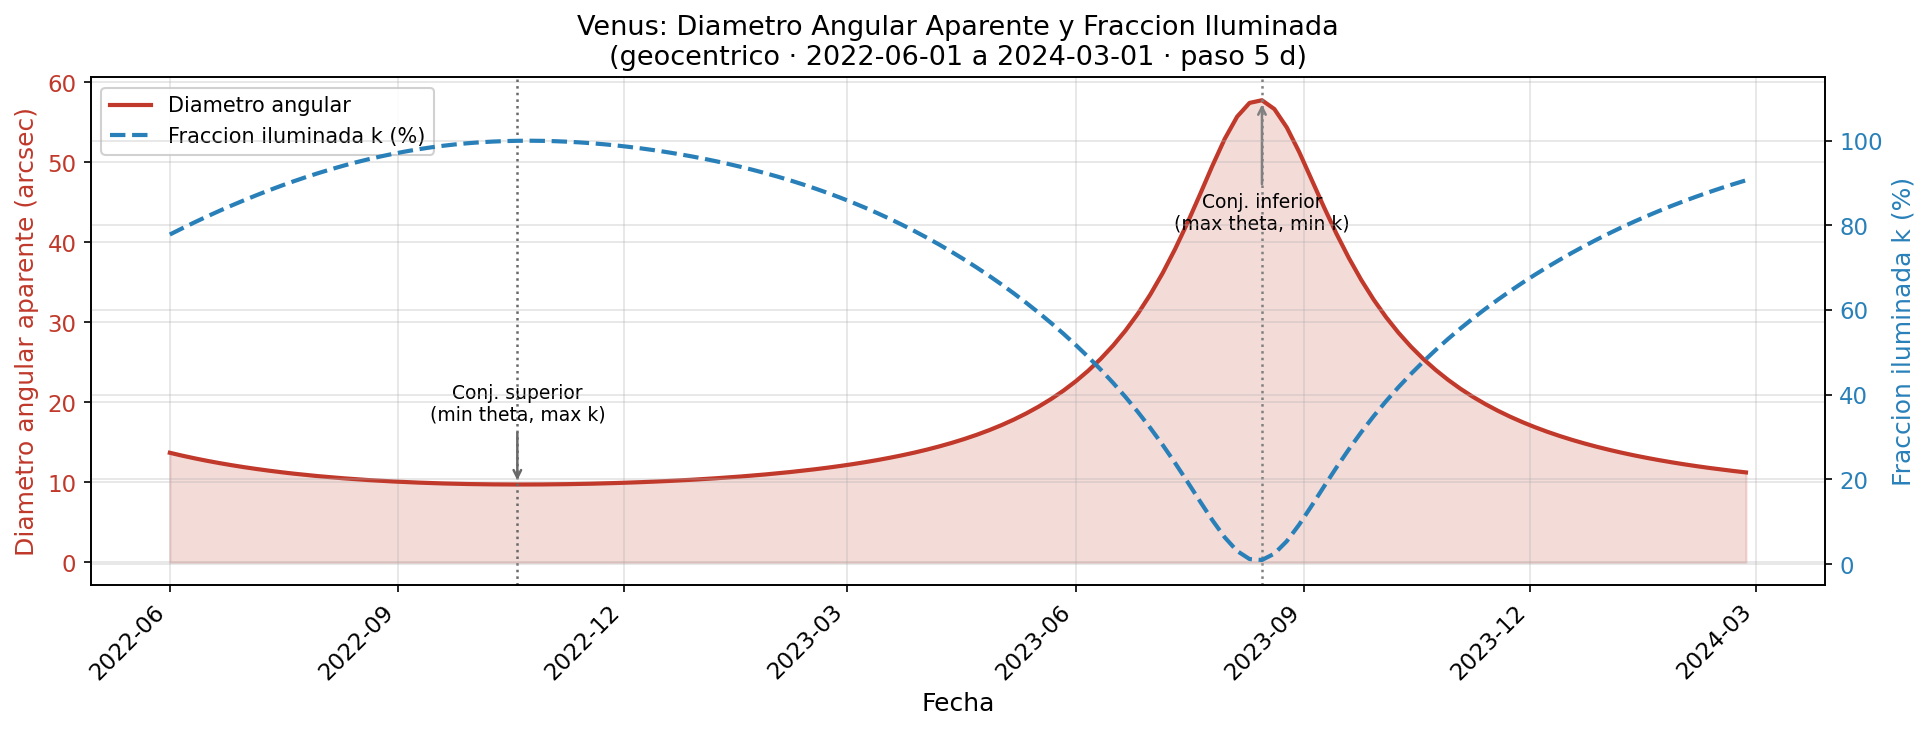
\includegraphics[width=0.94\textwidth]{imagenes/venus_diametro_iluminacion_vs_tiempo.png}
  \caption[Venus: diámetro e iluminación vs tiempo]{Evolución temporal del diámetro angular e iluminación de Venus. Se observa anti-correlación sistemática.
  Fuente: NASA/JPL Horizons \citep{Park2021}.}
  \label{fig:venus_tiempo}
\end{figure}

\begin{figure}[H]
  \centering
  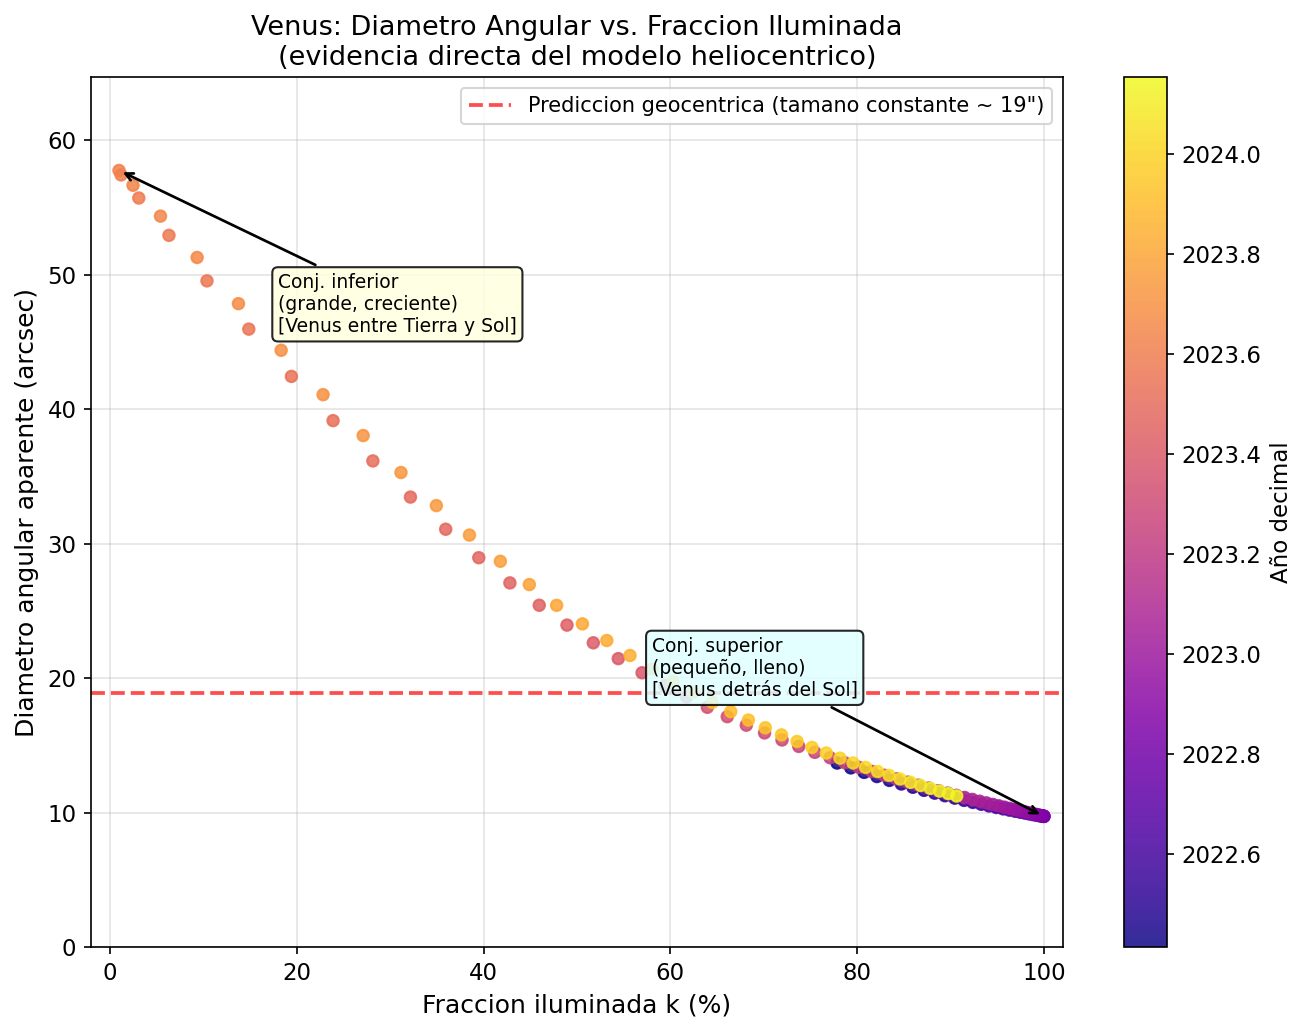
\includegraphics[width=0.84\textwidth]{imagenes/venus_diametro_vs_iluminacion.png}
  \caption[Venus: diámetro vs iluminación]{Relación entre diámetro angular y fracción iluminada de Venus.
  La tendencia negativa contradice la predicción geocéntrica de tamaño constante.
  Fuente: NASA/JPL Horizons \citep{Park2021}.}
  \label{fig:venus_diag}
\end{figure}

\begin{figure}[H]
  \centering
  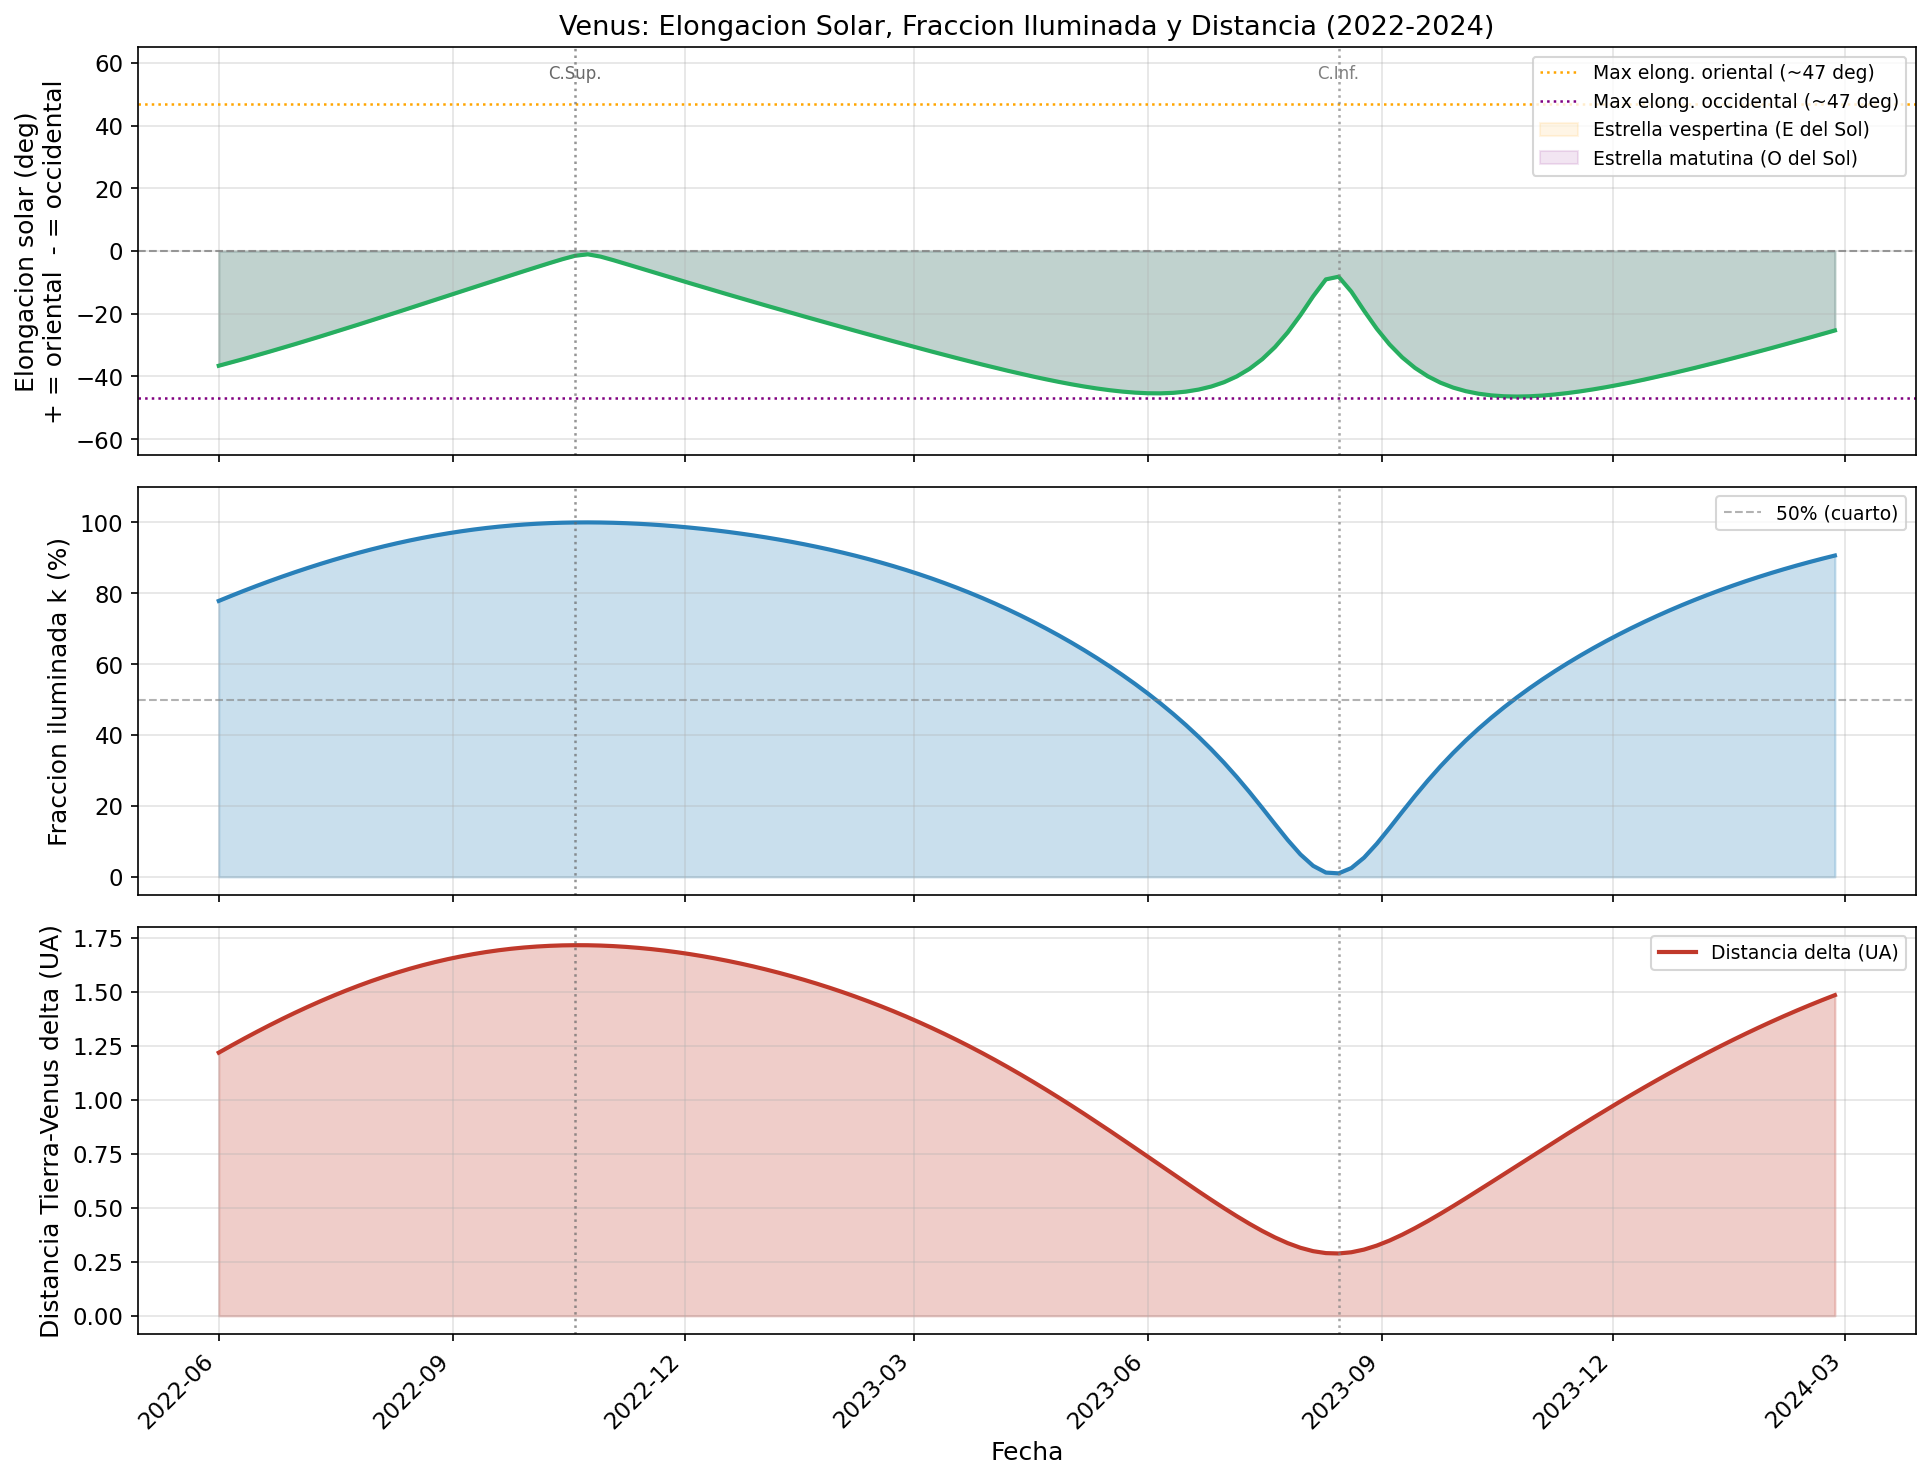
\includegraphics[width=0.94\textwidth]{imagenes/venus_elongacion_iluminacion_distancia.png}
  \caption[Venus: elongación, iluminación y distancia]{Elongación, fracción iluminada y distancia geocéntrica de Venus en el ciclo sinódico.
  La elongación se mantiene dentro de $\pm 47^\circ$.
  Fuente: NASA/JPL Horizons \citep{Park2021}.}
  \label{fig:venus_elong}
\end{figure}

\subsection{Marte: retrogradación}

La identificación cuantitativa del cuaderno reporta:
\begin{itemize}
  \item Oposición: 2027-02-18.
  \item Elongación solar: $174.96^\circ$.
  \item Diámetro angular: $13.81''$.
  \item Distancia geocéntrica: $0.6784$ UA.
  \item Retrogradación: 2027-01-09 a 2027-03-30 (80 días).
\end{itemize}

\begin{figure}[H]
  \centering
  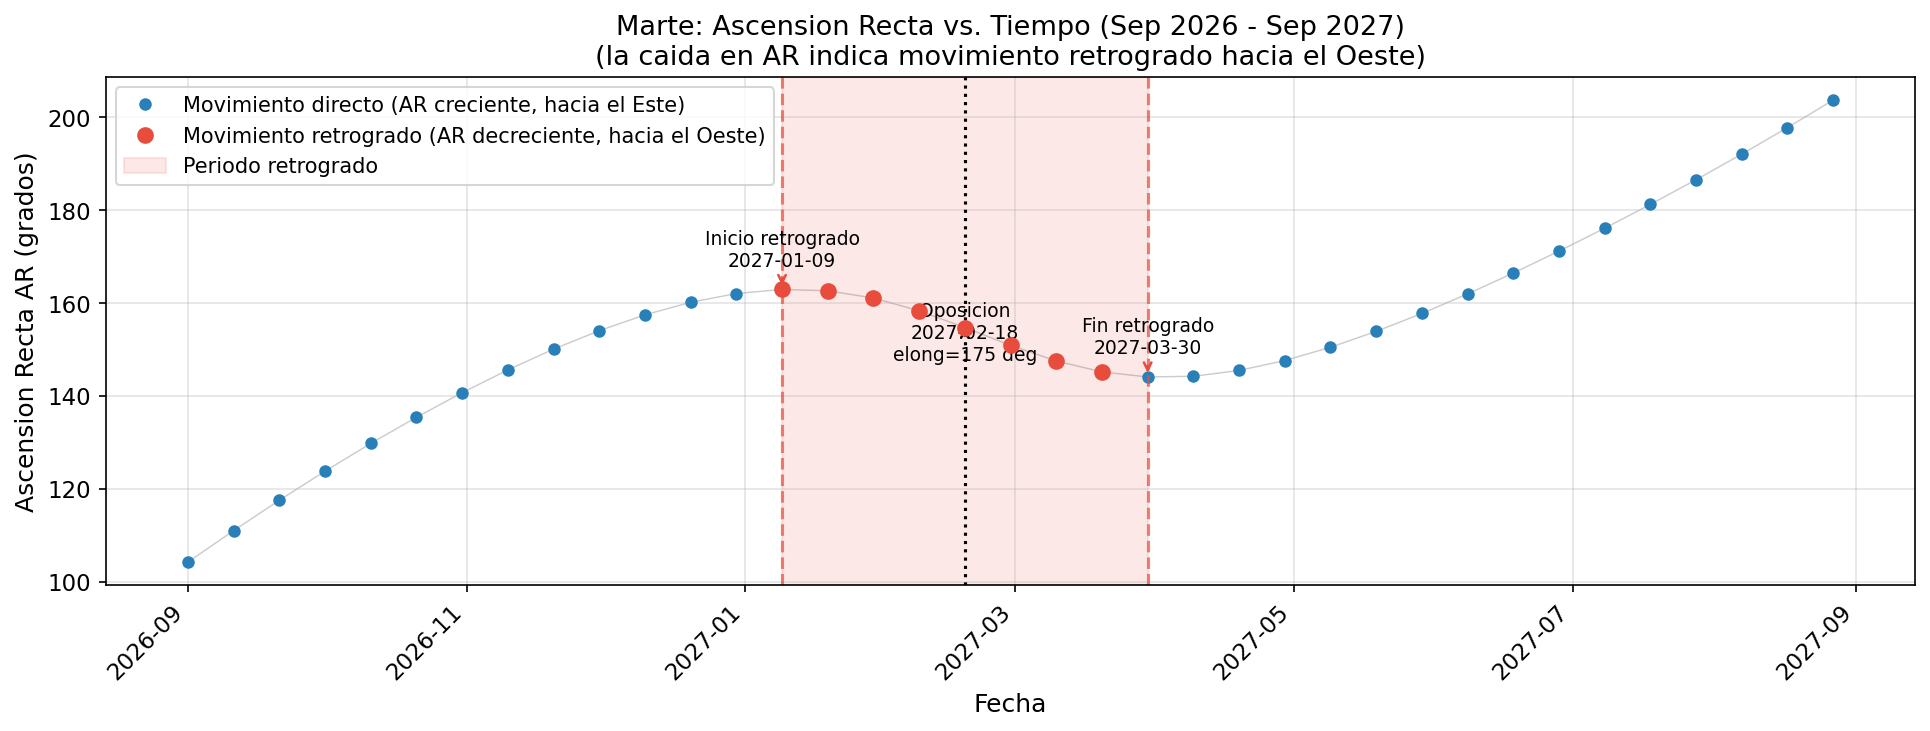
\includegraphics[width=0.94\textwidth]{imagenes/marte_RA_vs_tiempo.png}
  \caption[Marte: AR vs tiempo]{Ascensión recta de Marte en función del tiempo.
  El tramo con pendiente negativa marca la retrogradación.
  Fuente: NASA/JPL Horizons \citep{Park2021}.}
  \label{fig:marte_ra}
\end{figure}

\begin{figure}[H]
  \centering
  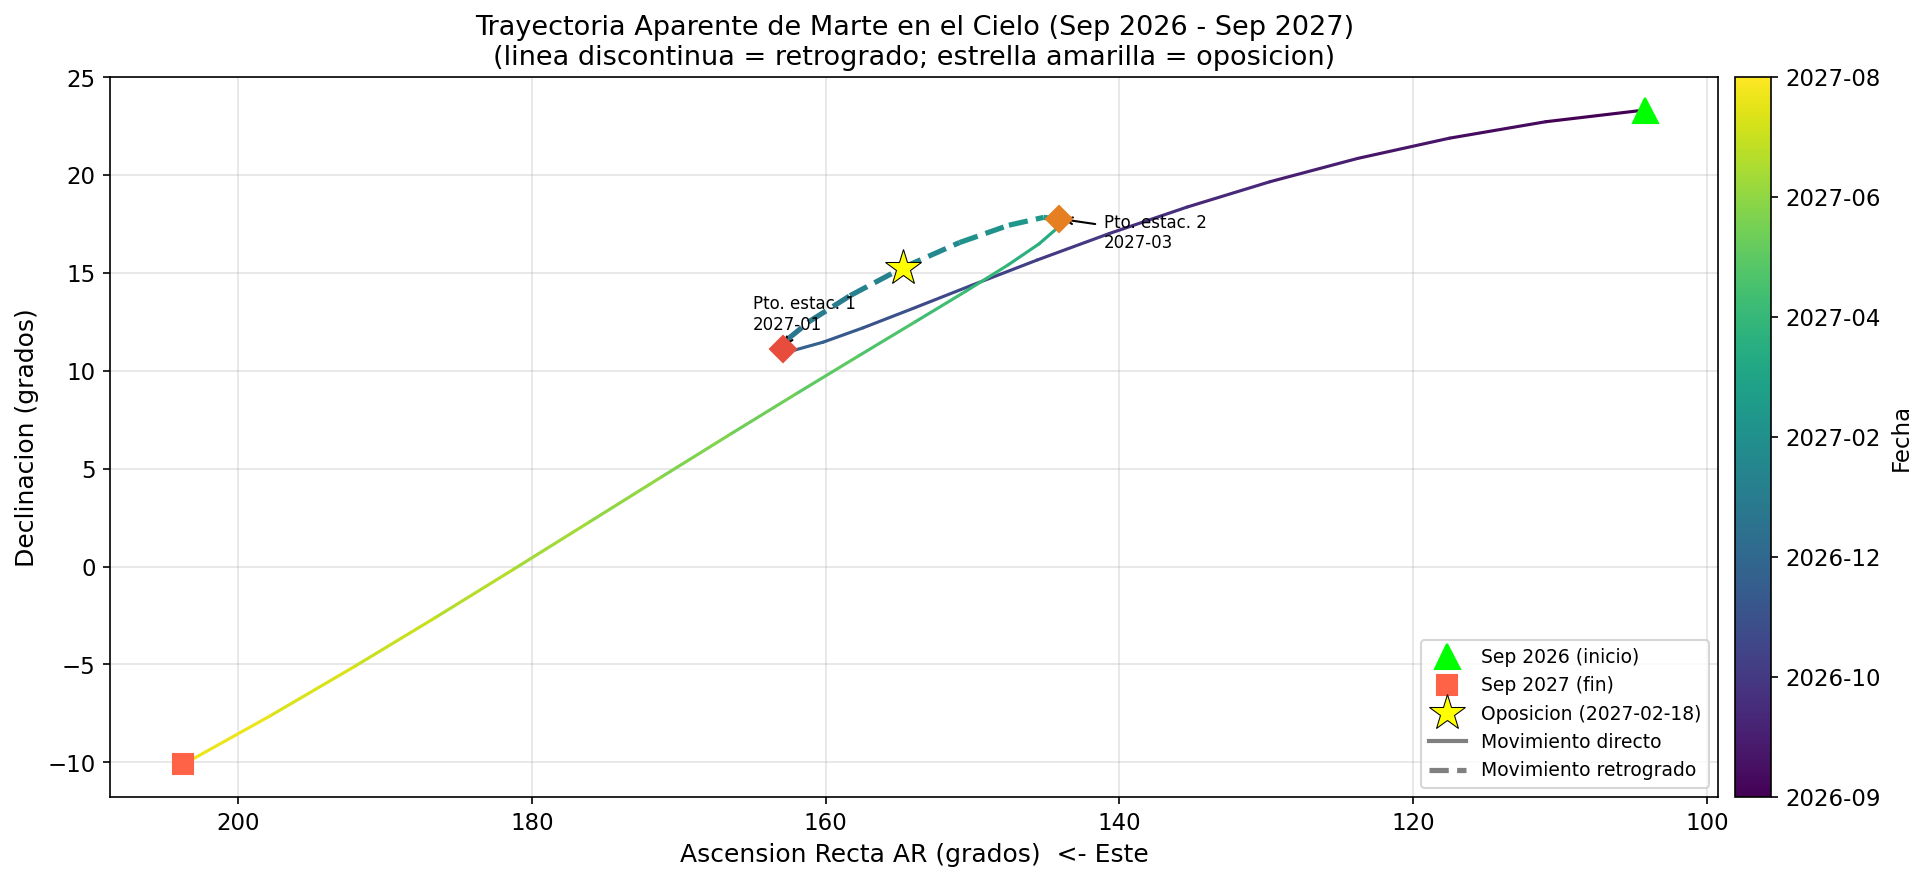
\includegraphics[width=0.94\textwidth]{imagenes/marte_trayectoria_cielo.png}
  \caption[Marte: trayectoria aparente en el cielo]{Trayectoria aparente de Marte sobre el fondo celeste durante 2026--2027.
  Se distingue el tramo retrógrado alrededor de la oposición.
  Fuente: NASA/JPL Horizons \citep{Park2021}.}
  \label{fig:marte_tray}
\end{figure}

\begin{figure}[H]
  \centering
  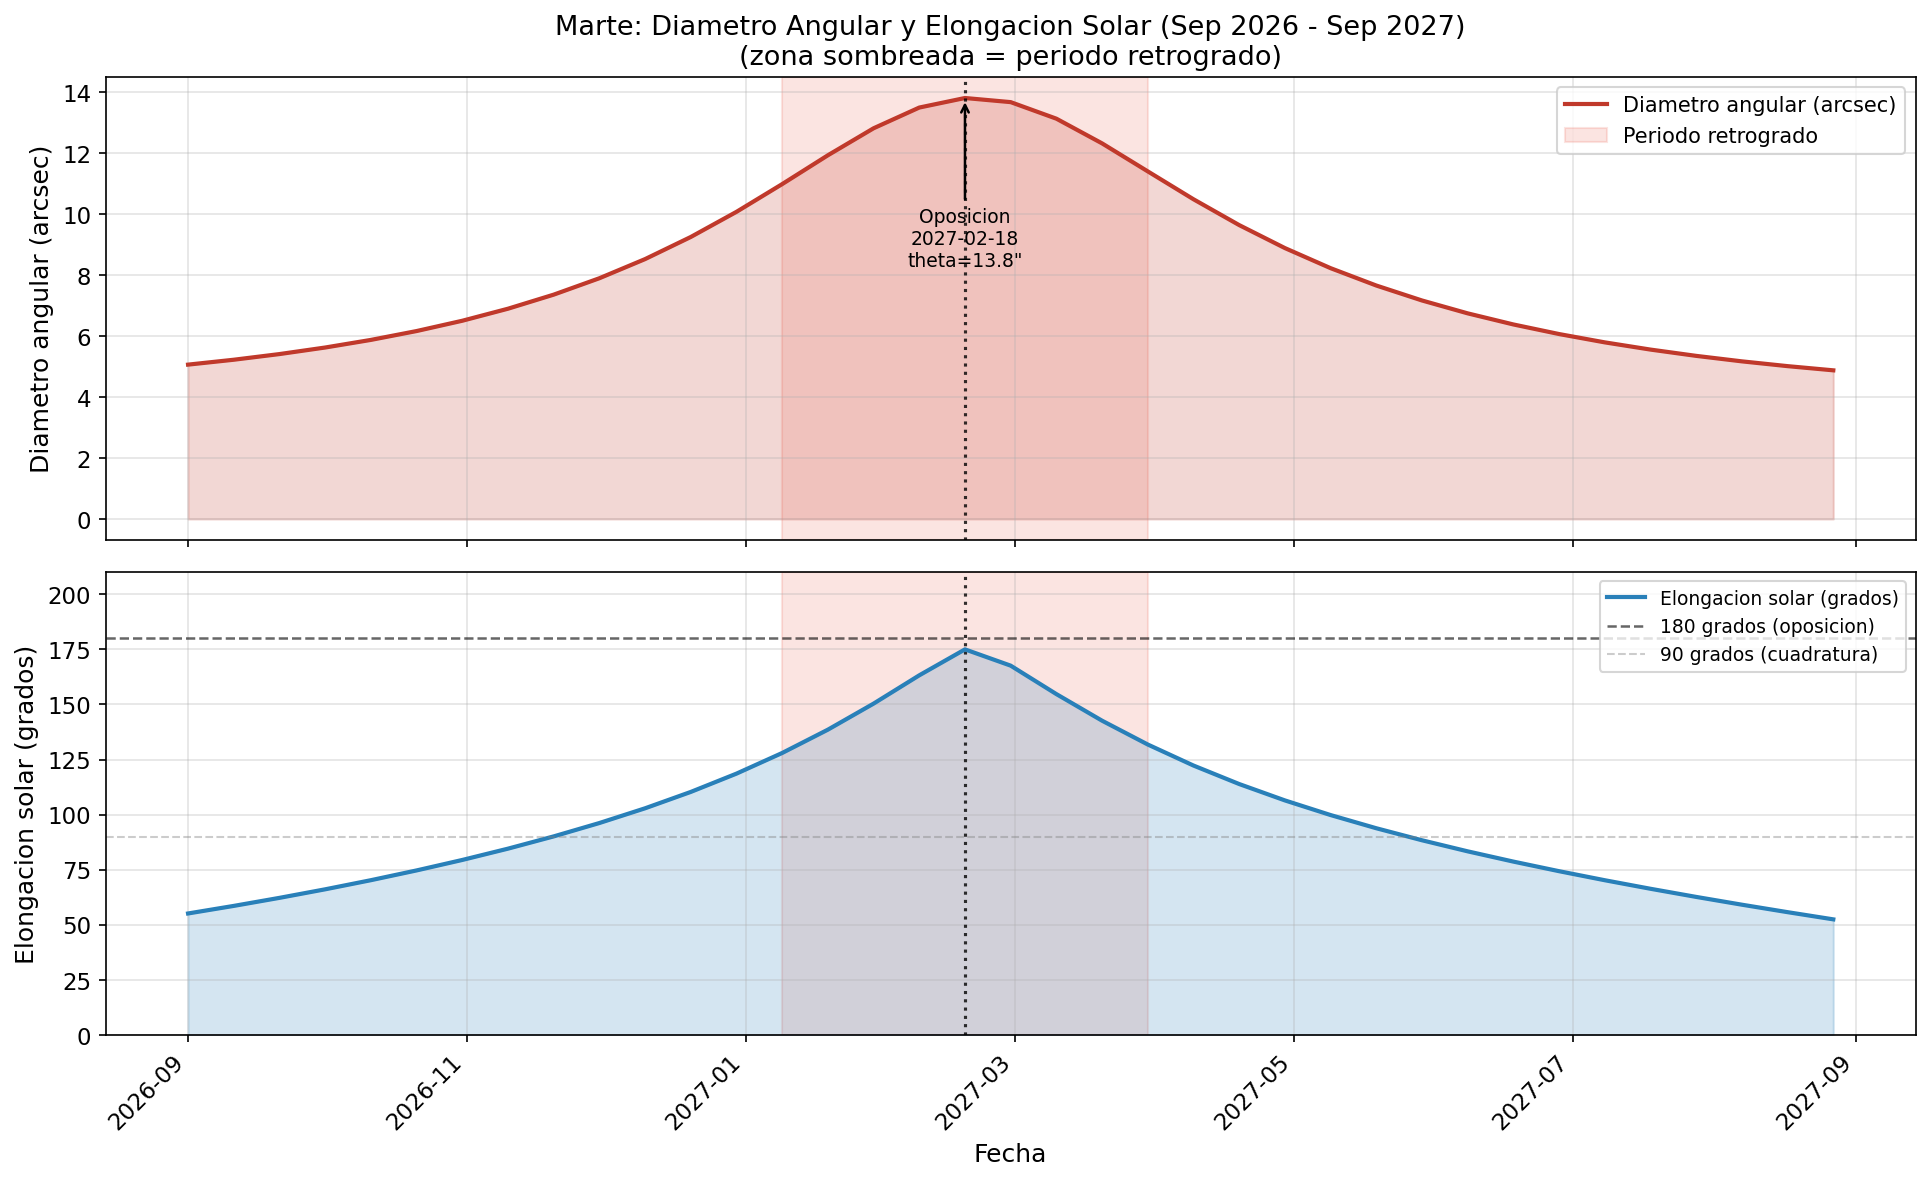
\includegraphics[width=0.94\textwidth]{imagenes/marte_diametro_elongacion.png}
  \caption[Marte: diámetro y elongación]{Diámetro angular y elongación de Marte durante el intervalo analizado.
  El máximo diámetro coincide con elongación cercana a $180^\circ$.
  Fuente: NASA/JPL Horizons \citep{Park2021}.}
  \label{fig:marte_diam}
\end{figure}

\section{Discusión}

Las observaciones de Venus reproducen la evidencia histórica de Galileo: fases
completas y variación grande de tamaño angular, incompatibles con el esquema
ptolemaico pero esperadas en el heliocentrismo.

Para Marte, la inversión temporal en AR y su sincronía con la oposición muestran
que la retrogradación no es un cambio real en la órbita del planeta, sino una
proyección geométrica causada por el movimiento relativo Tierra--Marte.

\section{Conclusiones}

\begin{enumerate}
  \item El período sinódico calculado para Venus ($583.93$ días) y Marte
  ($779.92$ días) coincide con los valores esperados de mecánica celeste.
  \item En Venus se verificó una anti-correlación robusta entre iluminación y
  tamaño angular, junto con elongaciones acotadas a $\pm 47^\circ$.
  \item En Marte se midió una retrogradación de 80 días centrada en la oposición
  de febrero de 2027.
  \item Los resultados cuantitativos de la práctica son consistentes con el modelo
  heliocéntrico y refutan la interpretación geocéntrica clásica.
\end{enumerate}
